\documentclass[border=6pt]{standalone}
\usepackage{tikz}
\usepackage[edges]{forest}
\usetikzlibrary{arrows.meta,positioning,calc,decorations.pathreplacing,shapes.geometric}
\begin{document}
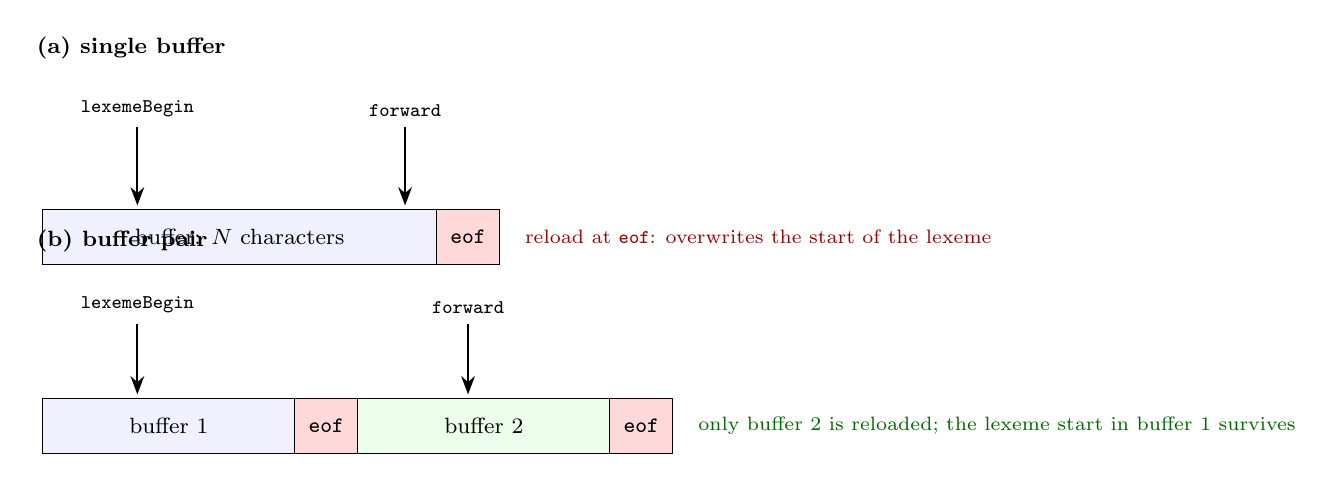
\begin{tikzpicture}[>=Stealth,font=\small,
 cell/.style={draw,minimum height=0.7cm,align=center,font=\footnotesize}]
\node[font=\footnotesize\bfseries,anchor=west] at (-0.2,3.4) {(a) single buffer};
\node[cell,minimum width=5.0cm,fill=blue!6] (s) at (2.5,1.0) {buffer: $N$ characters};
\node[cell,minimum width=0.8cm,fill=red!15] at (5.4,1.0) {\texttt{eof}};
\draw[->,thick] (1.2,2.4) node[above,font=\scriptsize]{\texttt{lexemeBegin}} -- (1.2,1.4);
\draw[->,thick] (4.6,2.4) node[above,font=\scriptsize]{\texttt{forward}} -- (4.6,1.4);
\node[font=\scriptsize,anchor=west,red!60!black] at (6.0,1.0) {reload at \texttt{eof}: overwrites the start of the lexeme};
\node[font=\footnotesize\bfseries,anchor=west] at (-0.2,0.95) {(b) buffer pair};
\node[cell,minimum width=3.2cm,fill=blue!6] (b1) at (1.6,-1.4) {buffer 1};
\node[cell,minimum width=0.8cm,fill=red!15] at (3.6,-1.4) {\texttt{eof}};
\node[cell,minimum width=3.2cm,fill=green!8] (b2) at (5.6,-1.4) {buffer 2};
\node[cell,minimum width=0.8cm,fill=red!15] at (7.6,-1.4) {\texttt{eof}};
\draw[->,thick] (1.2,-0.1) node[above,font=\scriptsize]{\texttt{lexemeBegin}} -- (1.2,-1.0);
\draw[->,thick] (5.4,-0.1) node[above,font=\scriptsize]{\texttt{forward}} -- (5.4,-1.0);
\node[font=\scriptsize,anchor=west,green!40!black] at (8.2,-1.4) {only buffer 2 is reloaded; the lexeme start in buffer 1 survives};
\end{tikzpicture}
\end{document}
